\section{Đánh giá nhận diện vật thể bằng YOLO}
\subsection{Thiết lập và phạm vi thống kê}
Hệ thống sử dụng YOLO11n với ngưỡng confidence 0,25, camera RGB độ phân giải $320\times240$, suy luận trên CPU và giới hạn 2 ảnh/giây. Robot thực hiện tuần tự 6 goal bằng node ROS 2.
Khoảng thống kê từ 09:36:12 đến 09:42:19 ngày 18/10/2026, tương ứng thời điểm gửi Goal 1 đến khi Goal 6 thành công. Log chỉ in khoảng một kết quả mỗi 2 giây. Có 160 mẫu log, gồm 109 mẫu rỗng và 51 mẫu có detection, tổng cộng 94 bounding box thuộc 9 lớp.
\textbf{Số liệu dưới đây là số box trong mẫu log, không phải tổng detection của mọi khung hình hoặc số vật thể duy nhất.} Một vật thể có thể được đếm nhiều lần khi xuất hiện ở nhiều mẫu.
\begin{table}[htbp]\centering\small
\caption{Thống kê lớp nhận diện trong 160 mẫu log của chuỗi 6 goal.}
\begin{tabular}{lrrcl}\hline
Lớp & Số box & Số mẫu & Conf. min--max & Ảnh đối chiếu \\ \hline
chair & 36 & 13 & 0.25--0.41 & Sai (ảnh mẫu) \\
person & 32 & 31 & 0.30--0.90 & Đúng (ảnh mẫu) \\
cup & 15 & 5 & 0.25--0.39 & Sai (ảnh mẫu) \\
airplane & 4 & 4 & 0.39--0.39 & Sai (ảnh mẫu) \\
umbrella & 3 & 3 & 0.27--0.37 & Sai (ảnh mẫu) \\
fire hydrant & 1 & 1 & 0.28--0.28 & Chưa tin cậy \\
refrigerator & 1 & 1 & 0.33--0.33 & Sai (ảnh mẫu) \\
tv & 1 & 1 & 0.29--0.29 & Sai (ảnh mẫu) \\
skateboard & 1 & 1 & 0.55--0.55 & Sai (ảnh mẫu) \\
\hline\end{tabular}\end{table}
Kết luận đúng/sai chỉ áp dụng cho các ảnh đã kiểm tra. Chưa gán nhãn từng box trong toàn bộ video nên không tính precision, recall hay mAP. Confidence trên ảnh minh họa có thể khác thống kê log vì ảnh được trích tại thời điểm lân cận.
\subsection{Đối chiếu ảnh thực nghiệm}
\begin{figure}[htbp]\centering
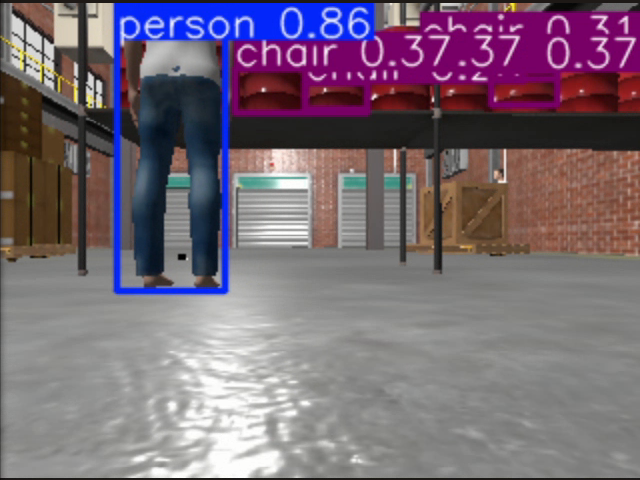
\includegraphics[width=0.72\linewidth]{evidence/chair_camera.png}
\caption{chair: Nhãn chair bao quanh các thùng đỏ trên kệ, không phải ghế.}
\end{figure}
\begin{figure}[htbp]\centering
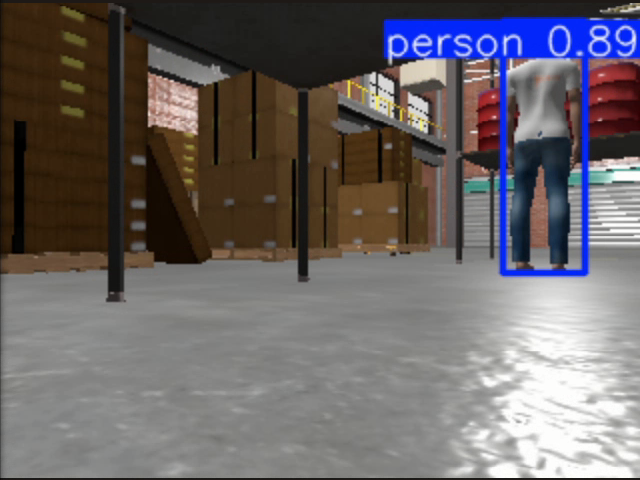
\includegraphics[width=0.72\linewidth]{evidence/person_camera.png}
\caption{person: Mô hình người có hình dạng, vị trí và bounding box phù hợp. Chưa gán nhãn thủ công toàn bộ các box person.}
\end{figure}
\begin{figure}[htbp]\centering
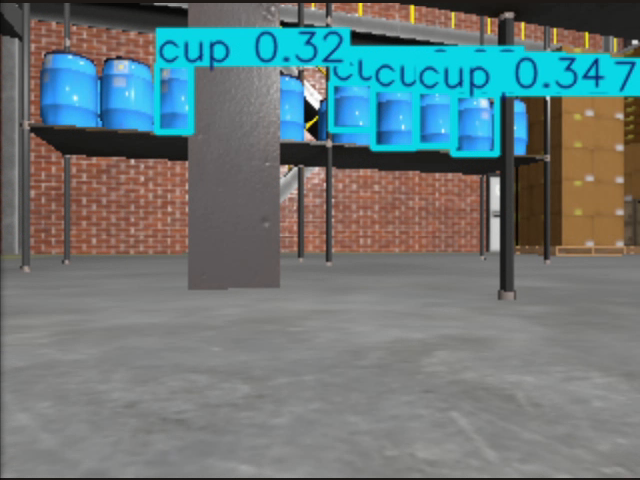
\includegraphics[width=0.72\linewidth]{evidence/cup_camera.png}
\caption{cup: Nhãn cup bao quanh thùng chứa màu xanh trên kệ, không phải cốc.}
\end{figure}
\begin{figure}[htbp]\centering
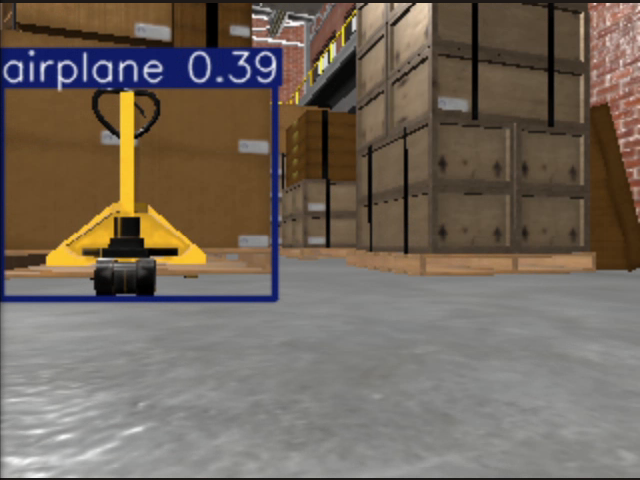
\includegraphics[width=0.72\linewidth]{evidence/airplane_camera.png}
\caption{airplane: Xe nâng tay màu vàng bị gán nhãn airplane.}
\end{figure}
\begin{figure}[htbp]\centering
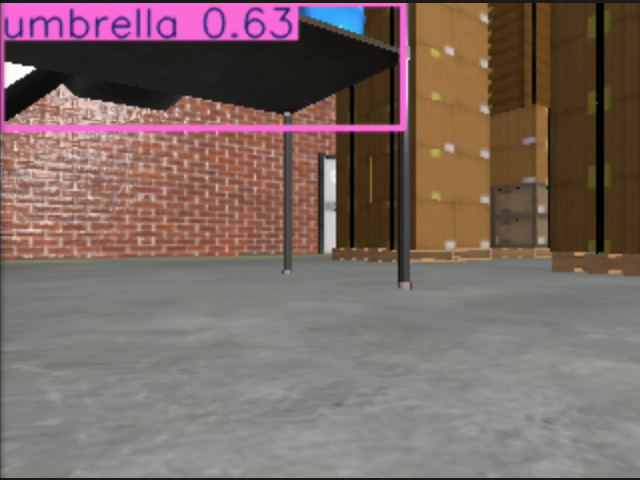
\includegraphics[width=0.72\linewidth]{evidence/umbrella_camera.png}
\caption{umbrella: Bộ phận màu đen phía trên ảnh bị gán nhãn umbrella; không phải ô.}
\end{figure}
\begin{figure}[htbp]\centering
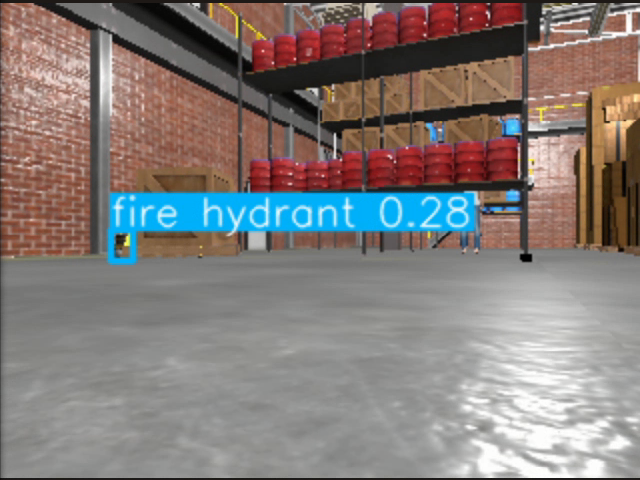
\includegraphics[width=0.72\linewidth]{evidence/fire_hydrant_camera.png}
\caption{fire hydrant: Box rất nhỏ gần chân kệ; ảnh không đủ rõ để xác nhận trụ nước. Chỉ có một mẫu log, confidence 0.28.}
\end{figure}
\begin{figure}[htbp]\centering
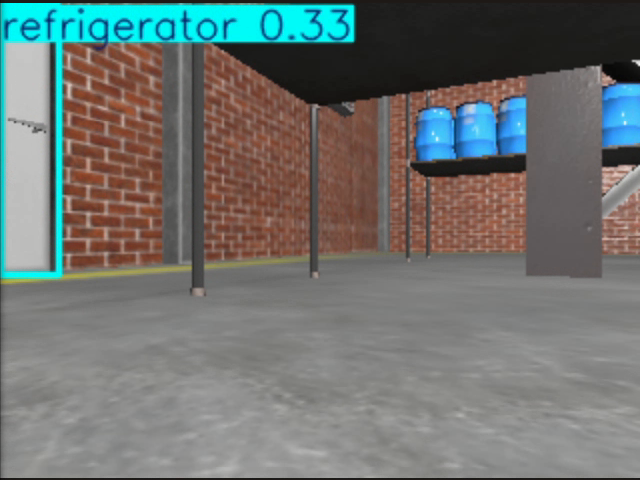
\includegraphics[width=0.72\linewidth]{evidence/refrigerator_camera.png}
\caption{refrigerator: Cột đứng của nhà kho bị gán nhãn refrigerator.}
\end{figure}
\begin{figure}[htbp]\centering
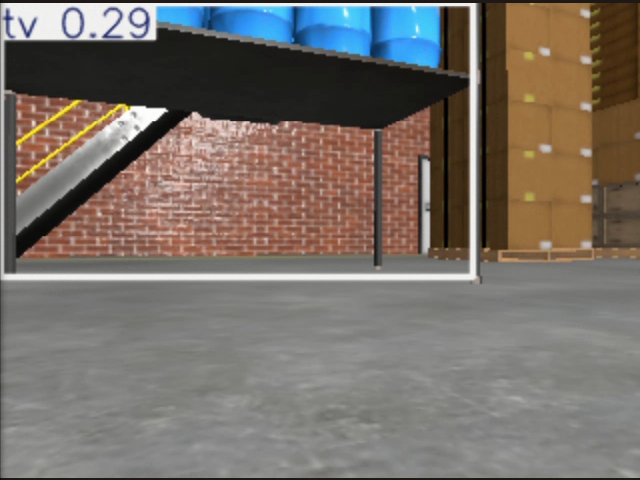
\includegraphics[width=0.72\linewidth]{evidence/tv_camera.png}
\caption{tv: Vùng kệ và nền nhà kho bị gán nhãn tv, không có màn hình TV trong box.}
\end{figure}
\begin{figure}[htbp]\centering
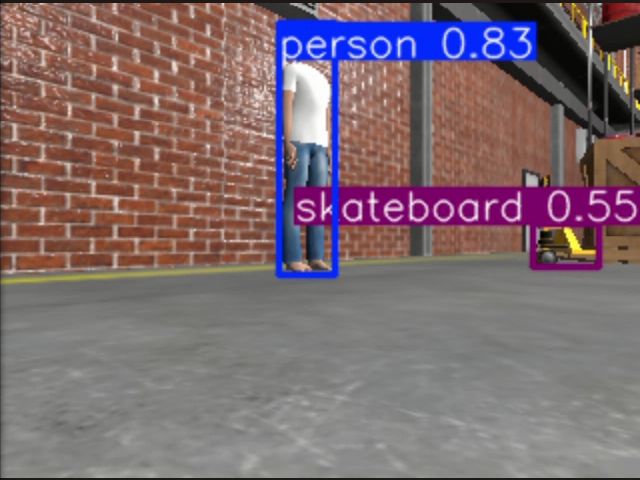
\includegraphics[width=0.72\linewidth]{evidence/skateboard_camera.png}
\caption{skateboard: Vật thể màu vàng sát nền (xe nâng tay trong kho) bị gán nhãn skateboard.}
\end{figure}
\clearpage
\subsection{Nhận xét và hạn chế}
Ảnh minh chứng cho thấy hệ thống phát hiện được mô hình người, đồng thời có nhiều nhận diện nhầm trên thùng chứa và kết cấu kho. Các mẫu rỗng không tự chứng minh bỏ sót vì có thể không có đối tượng phù hợp trong góc nhìn. Không suy ra số đối tượng thực tế bằng cách cộng số bounding box qua các mẫu.
Khác biệt ảnh mô phỏng so với dữ liệu huấn luyện, độ phân giải nhỏ, che khuất và góc nhìn thay đổi là các giả thuyết có thể ảnh hưởng kết quả; chưa có thí nghiệm riêng để định lượng từng yếu tố.
YOLO chạy song song để nhận diện và hiển thị, không điều khiển tránh vật cản. Kết quả 6/6 goal thành công xác nhận hoạt động navigation; không thay thế đánh giá độ chính xác của YOLO.
Cần lưu đầy đủ JSON và ảnh theo timestamp, gán nhãn một tập đánh giá đại diện, rồi so sánh các ngưỡng confidence hoặc mô hình trên cùng tập dữ liệu trước khi kết luận chất lượng được cải thiện.
